%%%%%%%%%%%%%%%%%%don't forget if needed %%%%%%%%%%%%%%%%%%%%%
%\section[toc version]{title version%
%              \sectionmark{head version}}
%\sectionmark{head version}
%%%%%%%%%%%%%%%%%%%%%%%%%%%%%%%%%%%%%%%%%%%%%%%%%%%%%%%%%%%%%%
\def\titcourt{Numerical simulation of natural convection flow in 2D square cavity}
\def\titlong{Numerical simulation of natural convection flow in 2D square cavity}
%%%%%%%%%%%%%%%%%%%%%%%%%%%%%%%%%%%%%%%%%%%%%%%%%%%%%%%%%%%%%%%%
\chapter[\titlong]{\titlong%
              \chaptermark{\titcourt}}
\chaptermark{\titcourt}
\label{chap-NATCONV}
%%%%%%%%%%%%%%%%%%%%%%%%%%%%%%%%%%%%%%%%%%%%%%%%%%%%%%%%%%%%%%%%
%%%%%%%%%%%%%%%%%%%%%%%%%%%%%%%%%%%%%%%%%%%%%%%%%%%%%%%%%%%%%%%%

We first focus on the capability of our code to deal with natural convection flow in square enclosures.
Internal convection flow is a relevant case to validate rigorously the Navier-Stokes-Boussinesq solver since publications related to the subject is very abundant in the literature.
A large number of benchmark solutions with reference to natural convection problem induced by temperature difference could be found in the literature. 
It is indeed central in a long list of engineering (circulations in building applications, double-wall insulations, solar collectors, etc.) and geophysical systems.

\noindent In this chapter, we are interested by natural convection of fluid in a square cavity differentially heated from the vertical walls.
The fluid temperature rises and its density decreases along the heated wall, convecting the fluid up to the point where it reaches the cold wall, during which the reverse process occurs. 
This two simultaneous opposing effects create a recirculation cell within a stationary zone in the center.

We solve the system of Eqs. \ref{eq-qmvt} - \ref{eq-energ}, with $A(\theta) = 0$ in the momentum equation and $S(\theta) = 0$ in the energy equation.
Linear and non-linear expressions of the buoyancy force $f_B(T)$ are investigated, by simulating the natural convection of air and the natural convection of water.
Natural convection of water exhibits actually a non-linear variation of the density with a maximum value around $T=4^o C$, while a linear variation is generally assumed for the natural convection of air in the Boussinesq approximation.
We consider a square enclosure of height $H$. 
Physical properties of air and water are listed in Tab. \ref{tab-param-phys-air}.
\begin{table}[!ht]
   \begin{center}
      \begin{tabular}{*{8}{cl}}
         
        & $\rho$ &$ \mu$ & $c_p $ & $k$ & $\alpha $ & $\beta$ \\
        & kg/m$^3$& kg/(m s) & J/(kg K) & W/(m K) & m$^2$/s & 1/K \\
         \hline
        Air & 1.177 & 1.85 $\cdot 10^{-5}$  & 1006 & $0.0262$ & $2.22 \cdot 10^{-5}$ & $3.4 \cdot 10^{-3}$ \\
        Water & 999.84 & 1.003 $\cdot 10^{-3}$  & 4182 & $0.578$ & $1.33 \cdot 10^{-7}$ & $6.91 \cdot 10^{-5}$
      \end{tabular}
   \end{center}
   \caption{Physical parameters of air and water at $T = 300K$ used in our simulations. $\Prd = 0.71$ (for air) and $\Prd = 6.99$ (for water).}
   \label{tab-param-phys-air}
\end{table}

\noindent Isothermal boundary conditions are applied to the vertical walls and adiabatic boundary conditions to the upper and lower walls.
Quantitative and qualitative validations are carried out as following:
\begin{enumerate}[label=(\roman*)]
\item \textbf{Natural convection of air without obstacle}: the velocity profile along symmetry lines, the maximum value of $u_{max}$ at mid-domain ($x=0.5$) and location $Y$ of this maximum  are compared with the spectral-accurate simulations by \cite{LeQuere91} in Sec. \ref{sub-diff-heated}, 
\item \textbf{Natural convection of air with heated obstacle}: transversal velocity profile along the  horizontal symmetry lines is compared with numerical results of \cite{Raluca2013} 
in Sec. \ref{sub-2D-OBSTACLE}, 
\item \textbf{Natural convection of water}: temperature profile along the horizontal symmetry line is compared with numerical results of \cite{Kowalewski-2003} in Sec. \ref{sec: natconv-water}.

\end{enumerate}

\section{Natural convection of air}\label{sec: natconv-air-2D}
We start by testing the Newton algorithm in Eq. \ref{eq-newton-C1} with respect to linear expression of $f_B(\theta)$  (see Eq. \ref{eq-RePr}). % by investigating simulations with linear expression of $f_B(\theta)$ as presented in Eq. \ref{eq-RePr}.
The classical problem of the thermally driven square cavity with adiabatic top and bottom walls is of interest.
We consider a cavity of height $H = 0.1$ m, initially filled with motionless air and a linear distribution of the temperature. 
The dimensionless parameters describing the investigated configuration are based on the fluid properties presented in Tab. \ref{tab-param-phys-air}, mainly $\Prd = 0.71$.
Three $\Ray$ numbers are computed: $\Ray = 10^4, 10^5, 10^6$. 
The characteristic scales of the problem are 
\begin{equation} \label{eq-scale-air}
	L_{ref} = H, \quad T_{ref} = \frac{T_h + T_c}{2},
\end{equation}

\noindent and,
\begin{equation} \label{eq-scaling-3}
   V_{ref} = \frac{\nu_l}{H} \sqrt{\frac{\Ray}{\Prd}} 
   \quad \Longrightarrow \quad t_{ref} = \frac{H^2}{\nu_l} \sqrt{\frac{\Prd}{\Ray}} 
   \quad \Longrightarrow \quad \Rey = \sqrt{\frac{\Ray}{\Prd}}.
\end{equation} 

\noindent The left wall is heated with dimensionless hot temperature $\theta_h = 0.5$ and the right wall is cooled with $\theta_c = -0.5$ (resulting from Eq. \ref{eq-scale-air}). 
A homogenous Dirichlet boundary condition ($\vec u = 0$) is applied for the velocity.
It has been shown by \cite{LeQuere91} that the solution of the 2-D Boussinesq equation in this configuration becomes unsteady at $\Ray= 10^{8.5}$.
Therefore, steady state can be achieved for the chosen Rayleigh numbers.

The unsteady  and steady Navier-Stokes-Boussinesq equations, related to algorithms \ref{eq-Newton-algo} and \ref{eq-Newton-steady} are simulated.
The unsteady case is computed until the steady state with a single convection cell is reached, with a numerical tolerance of $10^{-9}$.
Besides, the steady case is performed using Rayleigh number continuation:
a smaller value of the Rayleigh number is set initially, and is then increased smoothly until reaching the correct value.
At each stage, the computation starts from the solutions obtained from the previous Rayleigh number simulation.

Two cases are carried out: \textbf{ i)} a differentially heated square cavity and \textbf{ ii)} a differentially heated cavity with inner heated obstacle.
For each of them, the horizontal and the vertical velocity profiles $u(y)$ and $v(x)$ at mid-domain ($y=0.5$ and $x=0.5$ respectively) are plotted and compared with numerical results by \cite{LeQuere91} and \cite{Raluca2013}. 
Moreover, for \textit{ i)} the maximum value $u_{max}$ and its location $Y$ are accurately compared with the solutions obtained by spectral accurate simulations by \cite{LeQuere91}.

\subsection{Differentially heated square cavity} \label{sub-diff-heated}

\begin{figure}[!ht]
	\begin{center}
		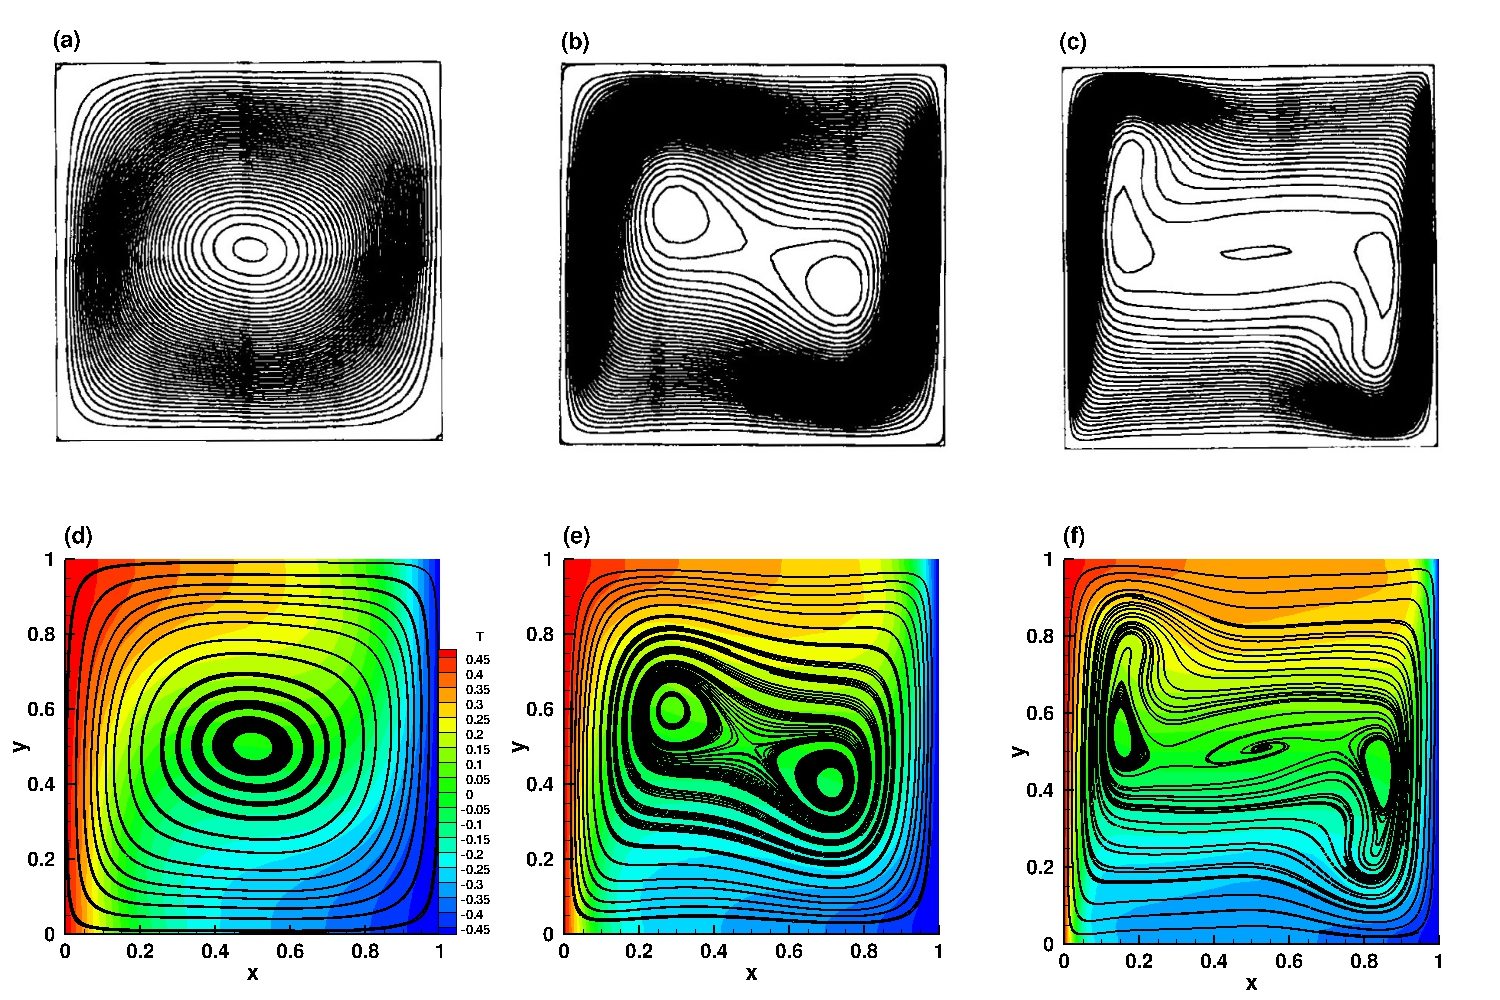
\includegraphics[width=0.98\textwidth]{\figpath/Fig_cap_natconv/NATCONV_air_valid-WS} 
	\end{center}
	\caption{Natural convection of air for $Ra$ ranging from $10^4$ to $10^6$ (from the left to the right) and $\Prd = 0.71$. Temperature fields and streamlines at the steady state. Panels (a) to (c) correspond to the benchmark solution of \cite{Wakashima-2004} (top). Panels (d) to (f) display our numerical results (bottom).}
	\label{fig-natconv-field}
\end{figure}

All computations in this section are performed with a fixed triangular mesh, generated by the Delaunay algorithm starting with {\em nbseg = 80} points on each side of the square.

Fig. \ref{fig-natconv-field} gives a comparison of the current simulation with the numerical results of \cite{Wakashima-2004}, who
used a fourth-order finite difference method for spatial discretization and third-order backward finite difference scheme for time integration.
The temperature distribution and the streamlines at the steady state are shown.
Our results match qualitatively well with the Benchmark solution.
The natural convection flow in the cavity is clearly enhanced when the $\Ray$ number is increased.
A single convection cell is observed in the center of the cavity for $\Ray = 10^4$ (Fig. \ref{fig-natconv-field}d) indicating that the heat transfer is merely bulk heat transfer.
Figs. \ref{fig-natconv-field}e and \ref{fig-natconv-field}f however exhibit stronger convection with more rolls, meaning that the heat transfer is dominated by boundary layer heat transfer.

More accurate validation is performed with respect to the spectral-accurate results of \cite{LeQuere91}.
We plot in Fig. \ref{fig-T1-prof} the horizontal (panel a) and the vertical (panel b)  profiles of the velocity and compare the current simulation with data extracted from  \cite{LeQuere91} for each of the three computed $\Ray$ numbers.
%Fig. \ref{fig-T1-prof} illustrates a comparison of the horizontal (Fig. \ref{fig-T1-prof}a) and the vertical (Fig. \ref{fig-T1-prof}b)  profiles of the velocity with data extracted from  \cite{LeQuere91} for each of the three computed $\Ray$ numbers.
Results from \cite{LeQuere91} are represented by solid lines and the current simulation by symbols.
A very good agreement can  be noticed for each case.

\begin{figure}
	\begin{center}
		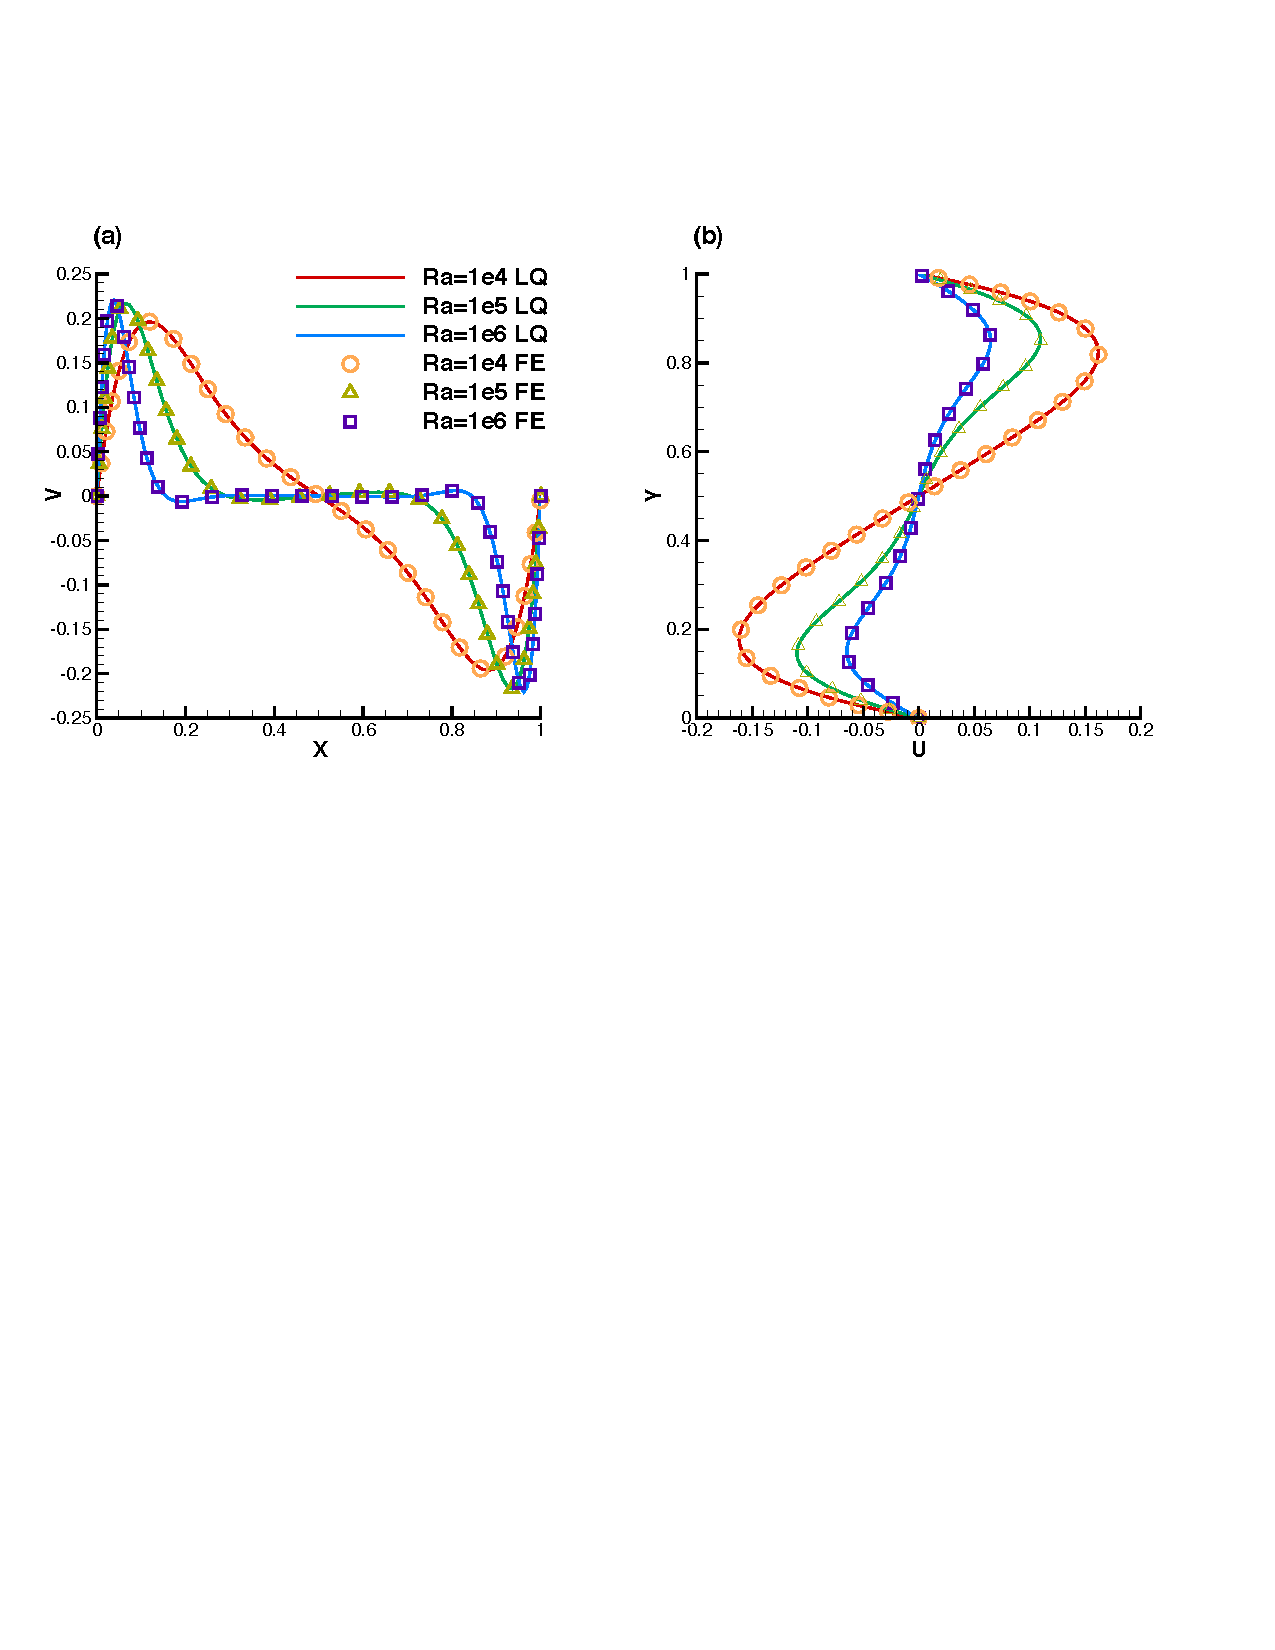
\includegraphics[width=0.98\textwidth]{\figpath/Fig_cap_natconv/Validation_Uprofile_LQ} 
	\end{center}
	\caption{Natural convection of air in a differentially heated cavity for $Ra$ ranging from $10^4$ to $10^6$ and $\Prd = 0.71$. (a) Transversal velocity profile along the  horizontal symmetry lines. (b) Longitudinal velocity profile along the vertical symmetry lines. Numerical results obtained using the present Newton method (symbols) with a mesh resolution of {\em nbseg} $=80$; comparison with the spectral-accurate simulations by \cite{LeQuere91} (solid lines).}
	\label{fig-T1-prof}
\end{figure}

The influence of the temperature difference $\delta T$ on the boundary layers are well illustrated by Fig.  \ref{fig-T1-prof}.
The scale analysis conducted in Sec. \ref{sec-bound-scal-anal} of Chapter \ref{chap-NSB} indicates a decreasing thickness of the boundary layer for an increasing value of $\Ray$ (see Eq. \ref{eq-corr-Low-Pr}). 
For $\Ray = 10^6$ a viscous boundary layer with a dimensionless thickness of order of $\delta_\nu \sim 0.02$ should be present close to the vertical walls.
Accordingly, the mesh resolution should allow to capture these structures.
%Also, from $\Ray = 10^5$ the fluid in the core of the cavity is relatively stagnant and thermally stratified.

\noindent A mesh convergence analysis is investigated in Fig. \ref{fig-mesh-analysis}. 
We compare the differences $\varepsilon_V = |V - V_{LQ}|$ along $x-$direction  and $\varepsilon_U = |U - U_{LQ}|$ along $y-$direction between the present simulation and the benchmark, with $V_{LQ}$ and $U_{LQ}$ the numerical solutions of   \cite{LeQuere91}.
Differences decrease when the mesh resolution is increased, validating hence the Newton method.
We can observe that errors lower than $6 \cdot 10^{-4}$ is obtained from $80 \times 80$ grid resolution.

\begin{figure}
	\begin{center}
		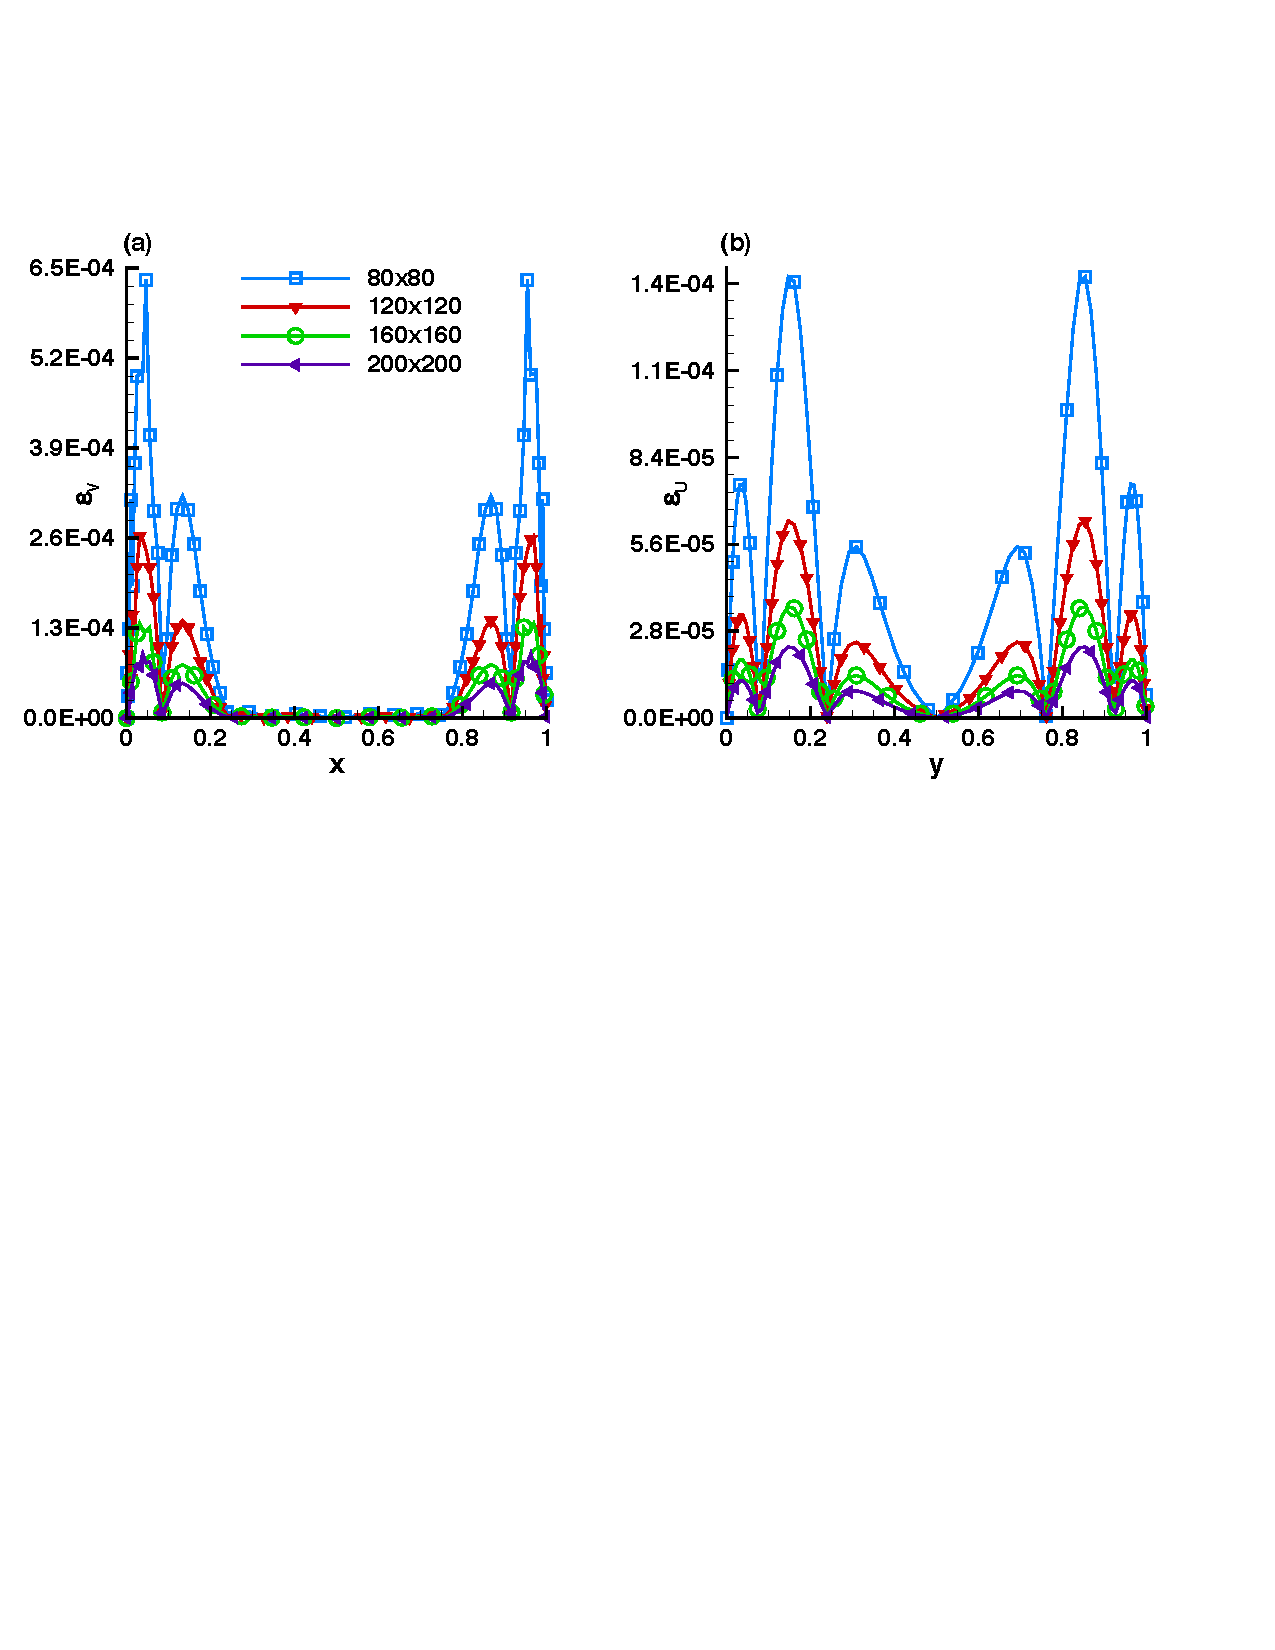
\includegraphics[width=\textwidth]{\figpath/Fig_cap_natconv/Mesh-conv} 
	\end{center}
	\caption{Natural convection of air. Mesh convergence analysis for $Ra=10^6$ and $\Prd = 0.71$. Comparison with \cite{LeQuere91}.}
	\label{fig-mesh-analysis}
\end{figure}


Tab. \ref{tab-valid-natconv} offers a quantitative assessment of the accuracy of the present Newton method. 
The values of $u_{max}$  and its location $Y$ are compared to reference values from \cite{LeQuere91}. 
The Newton method gives results very identical to reference values, with a relative difference less than $0.01 \%$ for the steady and the unsteady codes. 
The characteristics-Galerkin method is less accurate, but still offers reasonable agreement with reference values, within 2$\%$ relative error. 
We also recall that the characteristics method needs a very small time step for refined meshes ($\delta t = 8\cdot 10^{-5}$ for {\em nbseg} $= 80$), while the Newton method allows larger time steps ($\delta t = 1$ for {\em nbseg} $= 80$). % and consequently, converges faster to a steady state.
%It is worth noting, that the steady and the unsteady codes provide quasi-identical results.
\begin{table}%[!ht]
	\begin{center}
		\begin{tabular}{|l|c|l|l|}
			\hline
			\multicolumn{2}{|l|}{Run} & $u_{max}$ at x=$0.5$ (error) & $Y$ (error) \\
			\hline
			Reference values & spectral & 0.0648344           & 0.850 \\ \hline
			Char-Galerkin       & {\em nbseg} $=80$ & 0.0662229 (2.14 $\%$) & 0.856160 ( 0.72 $\%$) \\ \hline
			%\cite{dan-2014-JCP}              & nbseg$=80$ & 0.0650082 (0.26 $\%$) & 0.849906 ( 0.01 $\%$) \\ \hline
			Newton (Steady)        & {\em nbseg} $=80$ & 0.0648297 (0.007 $\%$) & 0.850394( 0.05 $\%$) \\ \hline
			Newton (Unsteady)        & {\em nbseg} $=80$ & 0.0648296 (0.007 $\%$) & 0.850532 ( 0.06 $\%$) \\ \hline
		\end{tabular}
	\end{center}
	\caption {Natural convection of air in a differentially heated cavity for $\Ray= 10^6$ and $\Prd = 0.71$. Maximum value $u_{max}$ of the horizontal velocity profile at mid-domain ($x=0.5$) and location $Y$ of this maximum. Comparison to reference values by \cite{LeQuere91}.}
	\label{tab-valid-natconv}
\end{table}

Finally, we compare the average Nusselt number at the left vertical wall with the reference values of \cite{de1983natural} and \cite{LeQuere91}.
From an engineering point of view, the most important characteristic of the flow is probably the rate of heat  transfer across the cavity.
In the next chapters, the Nusselt number will be largely used to compare the optimized configuration of a PCM either for melting or solidification cycle.
It is thus essential to ensure about the accuracy of the computed value of this parameter.
$N\!u$ is calculated as defined in Eq. \ref{eq-def-Nu}.
The comparison with \cite{de1983natural} is summarized below in Tab. \ref{tab-Nu-natconv}.
Excellent agreement with \cite{de1983natural} is obtained for each of the three $\Ray$ numbers, with a relative error lower than $0.01$.
It is important to note that we have exactly the same computed value of the Nusselt number as \cite{LeQuere91}.
%Also, the comparison with a P$_1$ discretization of the temperature have also been carried out and larger differences between \cite{de1983natural} and \cite{LeQuere91} was observed.
\begin{table}[!ht]
   \begin{center}
      \begin{tabular}{*{4}{cl}}
         
       $\Ray$ & $10^4$ &$ 10^5$ & $10^6 $ \\
         \hline
        \cite{de1983natural} & 2.245 & 4.523  & 8.927 \\
        \cite{LeQuere91} & - & - &  8.8252 \\
        Present simulation & 2.2448 & 4.5217  & 8.8252 \\
      \end{tabular}
   \end{center}
   \caption{Average Nusselt number on the vertical boundary of the cavity at $x=0$. Comparison with \cite{de1983natural} and \cite{LeQuere91} for $\Ray= 10^4$ to $10^6$.}
   \label{tab-Nu-natconv}
\end{table}


\subsection{Differentially heated cavity with inner heated square} \label{sub-2D-OBSTACLE}

\begin{figure}
	\begin{center}
		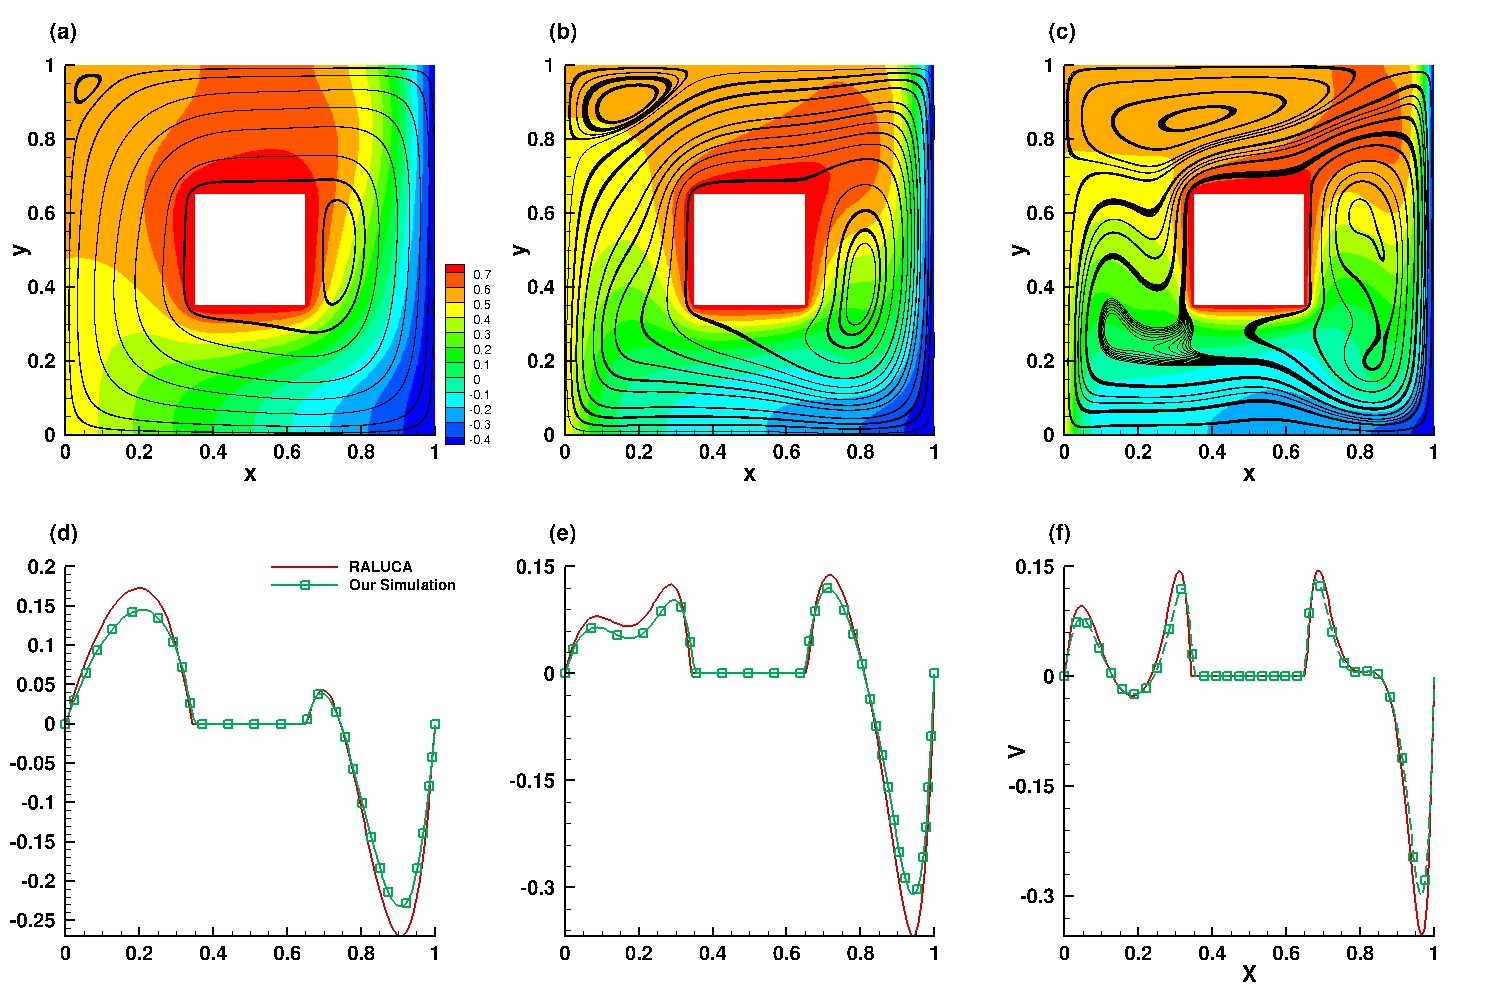
\includegraphics[width=\textwidth]{\figpath/Fig_cap_natconv/STA_validation_obstacle_3} 
	\end{center}
	\caption{Natural convection of air in a differentially heated cavity with inner heated square for $\Ray$ ranging from $10^4$ to $10^6$. Temperature field and streamlines (top) and transversal velocity profile along the  horizontal symmetry lines (bottom). Results obtained using the present Newton method (red solid line), with mesh resolution {\em nbseg} $=80$; comparison with the finite difference code of \cite{Raluca2013}.}
	\label{fig-obst-2D}
\end{figure}

Thermally driven cavity including heated square obstacle is computed in this section.
We consider the same configuration presented in Sec. \ref{sub-diff-heated} and a square involving isothermal boundary condition is added between the initial set up.
This kind of basic configuration could be representative of telecommunication outdoor cabinet applications, in which the use of passive cooling solutions have begun to be more and more investigated.
Indeed, inside an outdoor cabinet, electronic equipments generate heat when active and the study of the flow structures within the enclosure have attracted some considerations at the example of the experimental and numerical study of \cite{Raluca2013}.
Simplified model of cavity with rectangular heated obstacles have been investigated by \cite{Raluca2013} and will be reproduced in this section to test the robustness of our numerical algorithm.

A linear distribution of the temperature is imposed initially in the motionless air inside the cavity.
The obstacle is maintained at a dimensionless hot temperature $\theta_h = 0.8$ with a no-slip boundary condition for the velocity.
The solutions for $\Ray= 10^4$, $10^5$, $10^6$ and $\Prd = 0.71$ are compared with the result obtained by \cite{Raluca2013}, who used an immersed boundary method with a FD code using high order schemes for time and spatial discretization.

The temperature distribution in the cavity when the steady-state is reached, for each of the three computed $\Ray$ number, are reported in panels (a) to (c) of Fig. \ref{fig-obst-2D}.
The temperature gradient gives rise to a clockwise circulation and when $\Ray$ is increased, vertical thermal boundary layers form distinctly along the differentially heated sidewalls and the obstacle.
Consequently, 
higher is the Rayleigh number the more the hot temperature in the center of the domain is advected by the natural convection flow into the cold part of the cavity. 
Worth noting is the fact that at $\Ray = 10^6$ in panels (c) and (f), a stagnant fluid with a stratified temperature forms in a small portion of the fluid between the cold wall and the obstacle.

We assess a more accurate validation in panels (d) to (f) of Fig. \ref{fig-obst-2D}.
The transversal velocity profiles along the x-axis are plotted and compared with the numerical data of \cite{Raluca2013} for each cases. 
A good agreement can be observed with a relatively small differences between the extremum of the velocity while the trends of the velocity profile match well.

We have demonstrated in this part that the proposed Newton method offers an efficient way to solve the Navier-Stokes-Boussinesq system of equations for natural convection of air evolving a linear expression of $f_B(\theta)$.
A further difficulty will be introduced in the next section by including a non-linear expression of $f_B$ related to the natural convection of water.

\section{Natural convection of water inside a square cavity}\label{sec: natconv-water}
We perform in this section the natural convection of water in a differentially heated cavity. 
A further difficulty is introduced compared to the previous validations by taking into account non-linear variation of the density in the buoyancy force.
Pure water exhibits actually a non-linear density variation for $T< \celsm{10.2}$ with a maximum at $T_m= \celsm{4.0293}$. 
We use below the following density-temperature relationship  proposed in \cite{Gebhart1977}:
\begin{equation}\label{eq-dens-nonlin}
\rho(T)=\rho_m \left(1 - w \left|T - T_m\right|^q\right),
\end{equation}

\noindent with $\rho_m=999.972$ [kg/m$^3$], $w=9.2793\cdot 10^{-6}$ [($^\circ C)^{-q}$], and $q=1.894816$.
The bouyancy term $f_B = g(\rho_\vref-\rho)/\rho_\vref$ appearing in Eq. \ref{eq-momentum-conserv}  becomes after scaling:
\begin{equation}
f_B(\theta) = \frac{\Ray}{\Prd \, \Rey^2} \frac{1}{\beta \delta T}\, \frac{\rho(\theta_f)-\rho(\theta)}{\rho(\theta_f)},
\label{eq-fBnonlin}
\end{equation}

\noindent where $\beta=(1/\rho_m) \left(d\rho/dT\right)$ is the thermal expansion coefficient with the value $\beta=6.91 \cdot 10^{-5}$ [(K)$^{-1}$] \citep{Scanlon2004}.

We consider a cavity of height $H = 0.38$ m filled with liquid pure distilled water.
This problem was investigated experimentally and numerically by \cite{Giangi-2000,Kowalewski-1999,Kowalewski-2003}.
The height $H$ of the cavity is considered as a length scale of the problem $L_{ref} = H$. 
We choose $T_{ref} = T_h - T_c = 10 K$ in order to compare our simulation with the numerical results of \cite{Kowalewski-2003},
and define the following scaling:
\begin{equation} \label{eq-def-scal-1}
   V_{ref} = \frac{\nu_l}{H} 
   \quad \Longrightarrow \quad t_{ref} = \frac{H^2}{\nu_l}
   \quad \Longrightarrow \quad \Rey = 1.
\end{equation} 
The non-dimensional parameters describing the problem result from the physical properties of water in Tab. \ref{tab-param-phys-air}: $\Ray=2.518084\cdot 10^{6}$ and $\Prd=6.99$. %  (see also \cite{Kowalewski-2003} for physical details). % and $\Ste = 6.99$.

\noindent The initial temperature is linearly distributed with a hot (non-dimensional) temperature $\theta_h =1$ at the left wall and a cold temperature $\theta_c=0$ at the right wall. %, corresponding to dimensionless thermal boundary condition $\theta_h = 1$ and $\theta_c = 0$. 
The top and the bottom of the cavity are adiabatic and no-slip boundary condition $\vec u = 0$ is applied for the velocity.

The temperature field of the steady state is presented in Fig. \ref{fig-T1w-isoT}a.
Unlike the natural convection of air, in which two distinct boundary layers along the vertical walls and a stagnant and thermally stratified fluid in the core of the fluid flow were observed, an anomalous variation of the temperature is pointed out around the iso-line $\theta = \theta_m = 0.40293$ for the natural convection of water.
This anomalous thermal variation of water density, is clearly discernible in the streamline of the steady flow in Fig. \ref{fig-T1w-isoT}b.
Two recirculating zones are formed in the flow: a lower (abnormal) recirculation  in the vicinity of the cold wall where $\theta<\theta_m$ and an upper (normal) one where the density decreases with temperature ($\theta>\theta_m$).

Accounting for the foregoing comments, a greater mesh resolution should be applied around $\theta_m$.
We define thus a $\PP_1$ function $\Phi(\theta)$ defined by the following hyperbolic-tangent function similar to Eq. \ref{eq-Stanh}:

\begin{equation}
\Phi(\theta) =  \frac{1}{2}\left\{
1 + \tanh\left(\frac{\theta_m-\theta}{R_{\Phi}}\right)
\right\},
\label{eq-Stm}
\end{equation} 

\noindent with $R_{\Phi}=0.02$. 
The function $\Phi(\theta)$ and the two components of the velocity are used to compute the metric for the mesh adaptivity.
$\Phi(\theta)$ is used to track $\theta_m$ and the velocity allows to refine the boundary layer regions.
To reduce the impact of the interpolation on the global accuracy, since our algorithm is optimized to afford the mesh refinement every time step, we use both $\Phi(\theta^n)$ and $\Phi(\theta)^{n+1}$ in the adaptivity procedure.

\noindent The final mesh is displayed in Fig. \ref{fig-T1w-isoT}c.
The mesh is clearly refined along the line $\theta = \theta_m$ where  the structure and the extent of the two recirculating zones should be captured and along the vertical walls where the heat transfer is dominated by the boundary layer transfer.
Furthermore, as expected in the relatively stagnant fluid region, a coarser mesh is applied.

A more accurate comparison of the temperature profile along the horizontal symmetry line is given in Fig. \ref{fig-T1w-isoT}d. 
The temperature profile $\theta(x)$ along the horizontal symmetry line of the cavity is in good agreement with the numerical results   of \cite{Kowalewski-2003} obtained with FV and FD codes (FLUENT and FRECONV3V), commonly used in the heat transfer community. Differences are visible in the vicinity of the maximum density line, region where our mesh is well refined to capture the separation line between the two recirculation zones. It should be noted that the FLUENT simulations in \cite{Kowalewski-2003} are performed with a fixed uniform grid with $380\times380$ nodes, while our adapted grid has only 3422 triangles.

\begin{figure}
	\begin{center}
		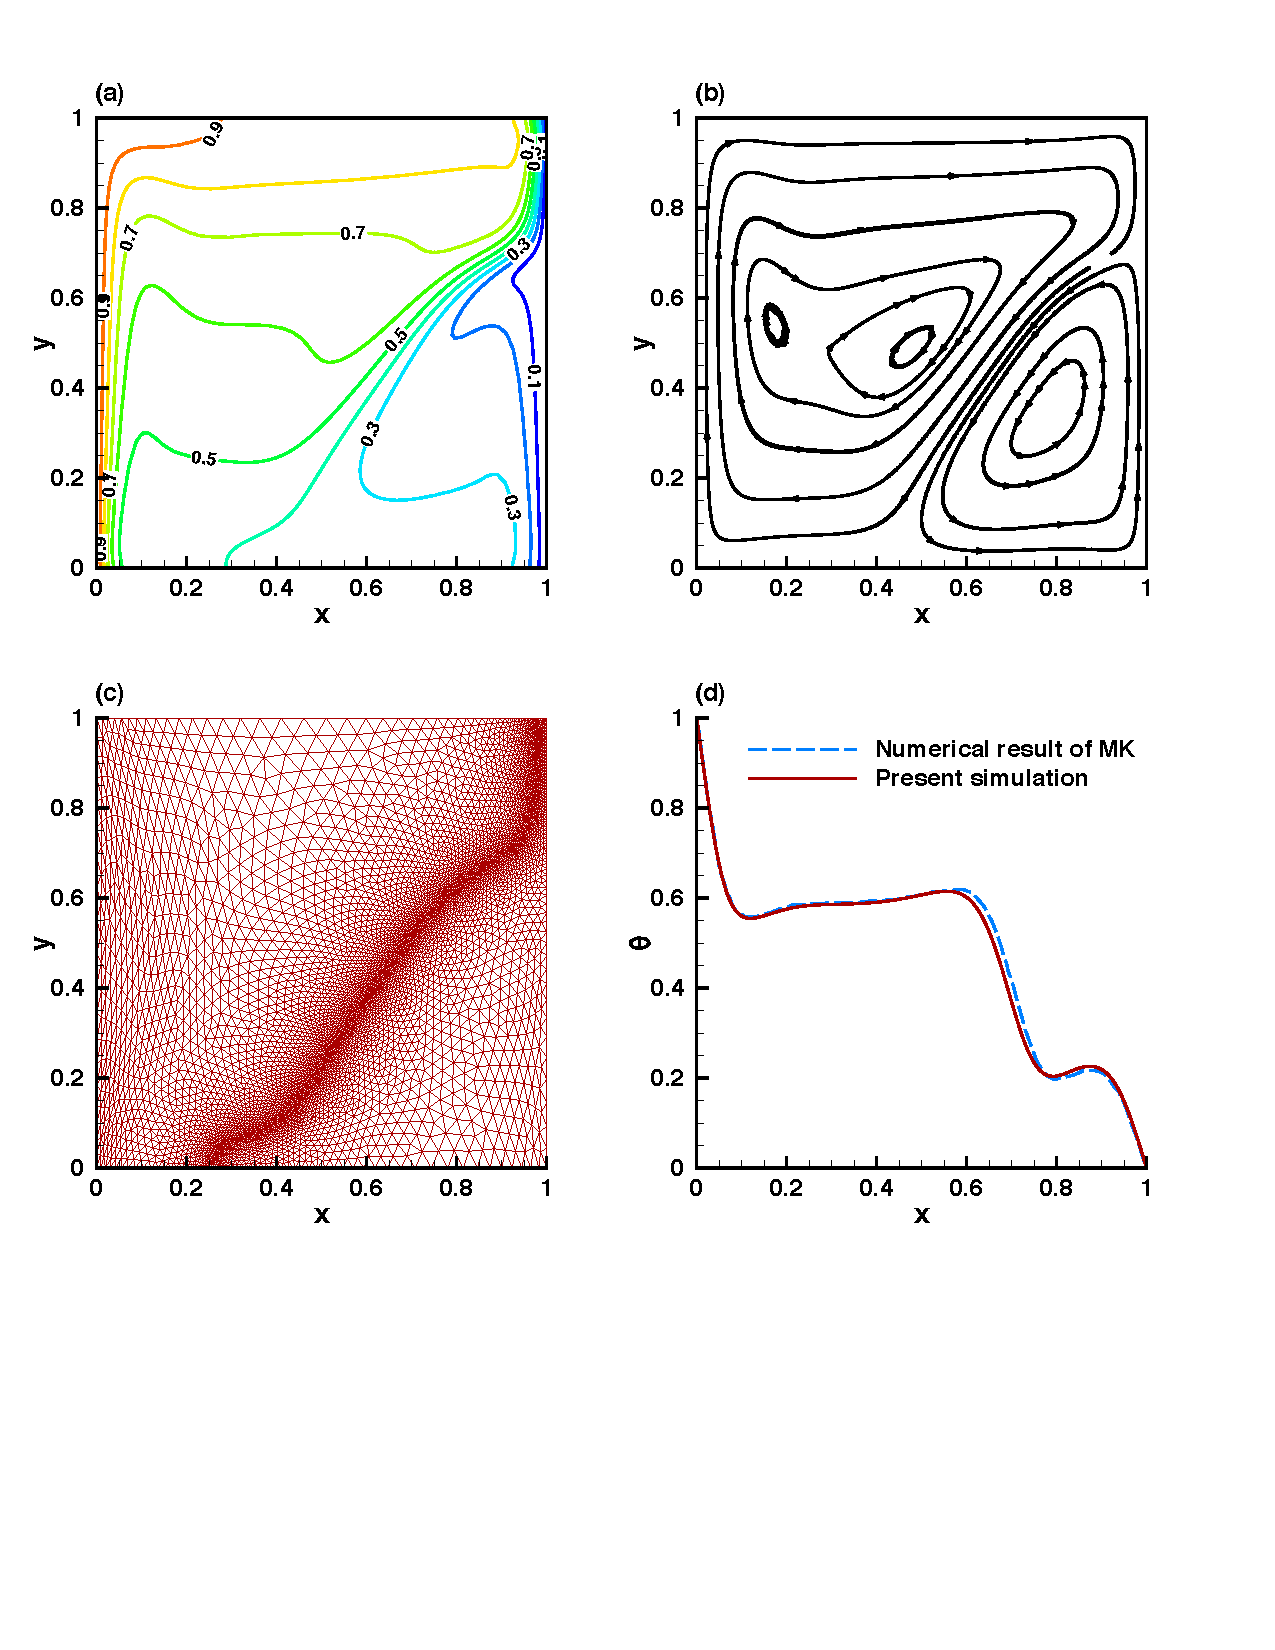
\includegraphics[width=0.98\textwidth]{\figpath/Fig_cap_natconv/WATER_convec_valid}
	\end{center}
	\caption{Natural convection of water in a differentially heated cavity with non-dimensional parameters: $\Ray=2.518084\cdot 10^{6}$ and $\Prd=6.99$. (a) iso-line of the temperature at the steady state. (b) Streamline of the steady flow. (c) Illustration of the mesh adaptivity: The mesh is refined along the dimensionless temperature iso-line $\theta = \theta_m$ due to the density variation. (d) Temperature profile along the horizontal symmetry line. Comparison with the numerical results of \cite{Kowalewski-2003}.}
	\label{fig-T1w-isoT} % label should be placed after the caption
\end{figure}

\newpage
\section{Concluding remarks}

We can conclude from Secs. \ref{sec: natconv-air-2D} and \ref{sec: natconv-water} that the developed Newton method is able to deal  efficiently with the two-dimensional Navier-Stokes-Boussinesq problem either with linear or non-linear formulations of the buoyancy force.

\noindent The natural convection of air including obstacle or not have proven very good agreement with the numerical solutions of \cite{LeQuere91} and \cite{Raluca2013}.
Excellent agreement with \cite{de1983natural} and \cite{LeQuere91} have also been observed for the value of the average Nusselt number at the heated wall. 

\noindent The challenging case of the natural convection of water have demonstrated the robustness of the 2D code. 
Good agreement with the numerical simulations of \cite{Kowalewski-2003} was noticed. 
The influence of the mesh adaptivity was clearly shown by the total grid number differences of order of $40$ between the present simulation and those of \cite{Kowalewski-2003} .
The refined mesh along the line $\theta_m$ have permitted to solve more accurately the structures and the extent of the two recirculating zones.

The description of the run presented in this chapter are summarized in Tab. \ref{tab-natconv-cases} for highest values of $\Ray$ numbers, mainly $\Ray = 10^6$.
The interest of solving the steady equation when steady state could be reached is clearly emphasised regarding the number of iterations and the CPU time.
$1,164$ iterations and $3162.86$ CPU seconds are indeed necessary to achieve the steady state with a tolerance of $10^{-6}$ for the natural convection of water by solving the unsteady equation,
while only $20$ iterations and $51.1662$ CPU seconds are needed with the steady algorithm.

\begin{table}[!ht]
\centering
\begin{tabular}{*{6}{c}}
  & Case & {\small Nb of iterations} & {\small Nb of triangles} & {\small Nb of d.o.f.} & {\small CPU time (s)}   \\
  \toprule 
  \multirow{2}{*}{Air} & unsteady & $164$ & $2,413$ & $16,133$ & $338.527$ \\
   & steady & $6$ & $2,312$ & $15,558$ & $14.0465$ \\
  \hline
  \multirow{2}{*}{Air with obstacle} & unsteady & $157$ & $3,489$ & $23,354$ & $436.405$ \\
  & steady & $6$ & $2,967$ & $19,933$ & $15.9369$ \\
  \hline
  \multirow{2}{*}{Water} & unsteady & $1,164$ & $3,422$ & $22,639$ & $3162.86$ \\
   & unsteady & $20$ & $2,960$ & $19,629$ & $51.1662$ \\

\bottomrule
 \end{tabular}
\caption{Description of the run of natural convection cases for $\Ray = 10^6$.}
\label{tab-natconv-cases}
\end{table}

We simulate in the next chapter the melting and the solidification of PCM.
Aside from the non-linear convection terms in the momentum and the energy Eqs. \ref{eq-qmvt} - \ref{eq-energ}, a further difficulty arise from the non-linearity introduced by the source term $\partial (CS)/\partial t$ in Eq. \ref{eq-energ}.
